We now present the inclusive study performed at NLO QCD, namely $\mathcal{O}(\alpha_s\alpha^6)$.

According to the results shown in Sec.~\ref{subsec:LOinclusive}, the VBS approximation at LO fails in the region $m_{jj} < 200$ GeV, $|\Delta y_{jj}| < 2$; moreover, we would like to validate this approximation (and its extension to $s$--channels inclusion) at the NLO accuracy.
Thus, we impose the same kinematic cuts shown in sec.~\ref{subsec:inputpar} relaxing the VBS cuts and asking for
\begin{equation}
	m_{jj} > 200 \,\textrm{GeV}\,,\qquad |\Delta y_{jj}| > 2\,.
\end{equation}
We compare three different predictions at NLO QCD: {\sc Bonsay} employs the VBS approximation ($|t|^2+|u|^2$), {\sc VBFNLO} adds the s--channel contributions ($|s|^2+|t|^2+|u|^2$) and {\sc Recola} employs full matrix--elements, adding also $t/u$ interferences, factorisable and non--factorisable QCD corrections to the leading electroweak order, as well as the EW correction to the $\mathcal{O}(\alpha_s\alpha^5)$ interference.
The total cross sections within the above mentioned kinematic cuts are shown in Tab.~\ref{tab:crosssecINCLUSIVE}.
\begin{table}[h!]
\centering
\begin{tabular}{c|c|c}
\bf Matrix--element & $\sigma_{\textrm{tot}}\,[\textrm{fb}]$ & $\delta$ \\
\hline
\hline
full &  1.8120 $\pm$ 0.0144 & - \\
\hline
$|t|^2 + |u|^2$ & 1.6292 $\pm$ 0.0001  &  -10 \% \\
\hline
$|s|^2 + |t|^2 + |u|^2$ & 1.7780 $\pm$ 0.0001  & -2 \%
\end{tabular}
\caption{\label{tab:crosssecINCLUSIVE}Total cross--sections at NLO QCD $\mathcal{O}(\alpha_s\alpha^6)$, with $m_{jj}>200$ GeV, $|\Delta y_{jj}|>2$.}
\end{table}
The VBS approximation for NLO QCD predictions (labelled by $|t|^2 + |u|^2$) gives a negative discrepancy of about 10 \% w.r.t the full calculation; the inclusion of $s$--channel diagrams improves the approximate prediction up to a 2 \% discrepancy.\\
These discrepancies are much more evident in differential cross--sections.\\
In Fig.~\ref{fig:mjjdyjj_1d_1} we show the distributions in the jet--jet invariant mass $m_{jj}$ and rapidity separation $\Delta y_{jj}$: at large $m_{jj}$ and large $\Delta y_{jj}$ the VBS approximation and its $s$--channel extension agree with the full calculation within few percents.
\begin{figure}[hbt]
\centering
{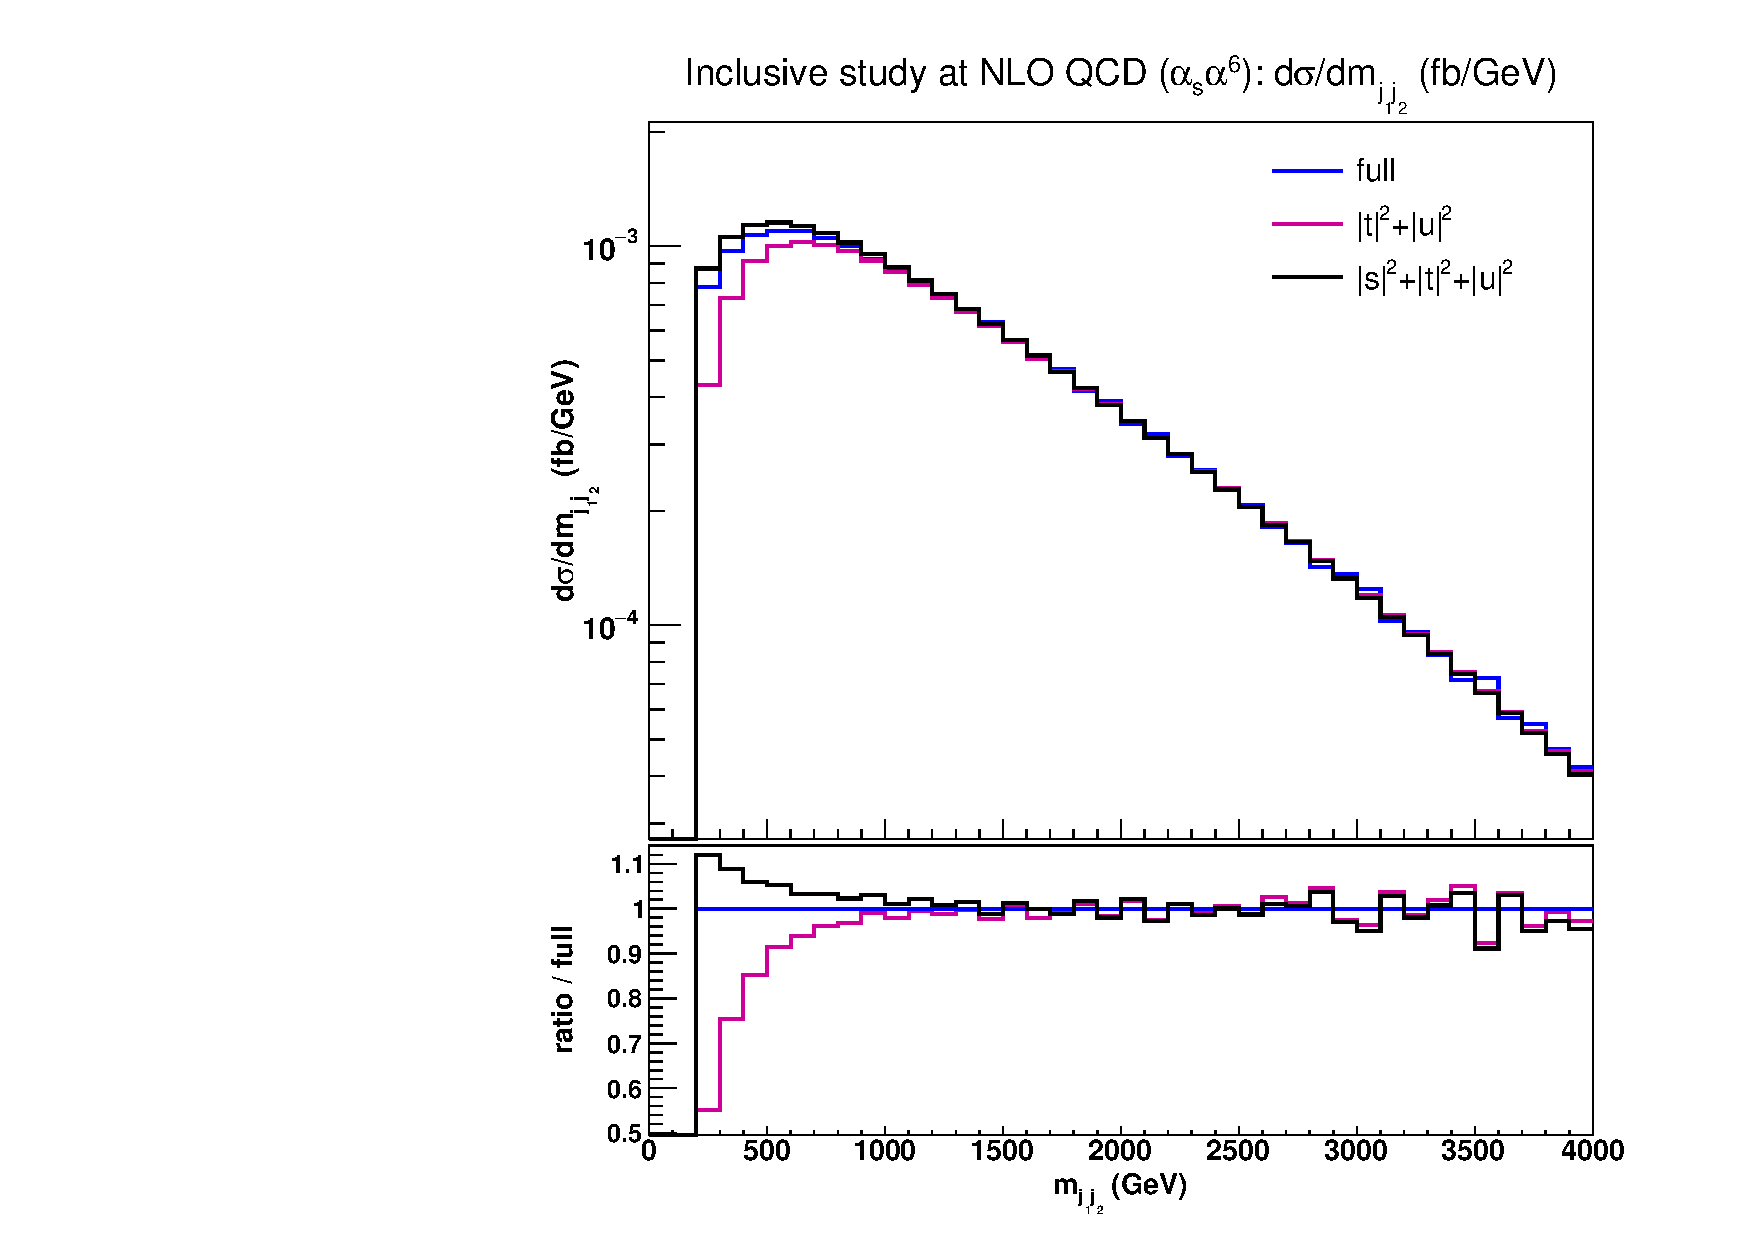
\includegraphics[scale=0.35]{figures/scanfigures/mjj_nlo.pdf}}
{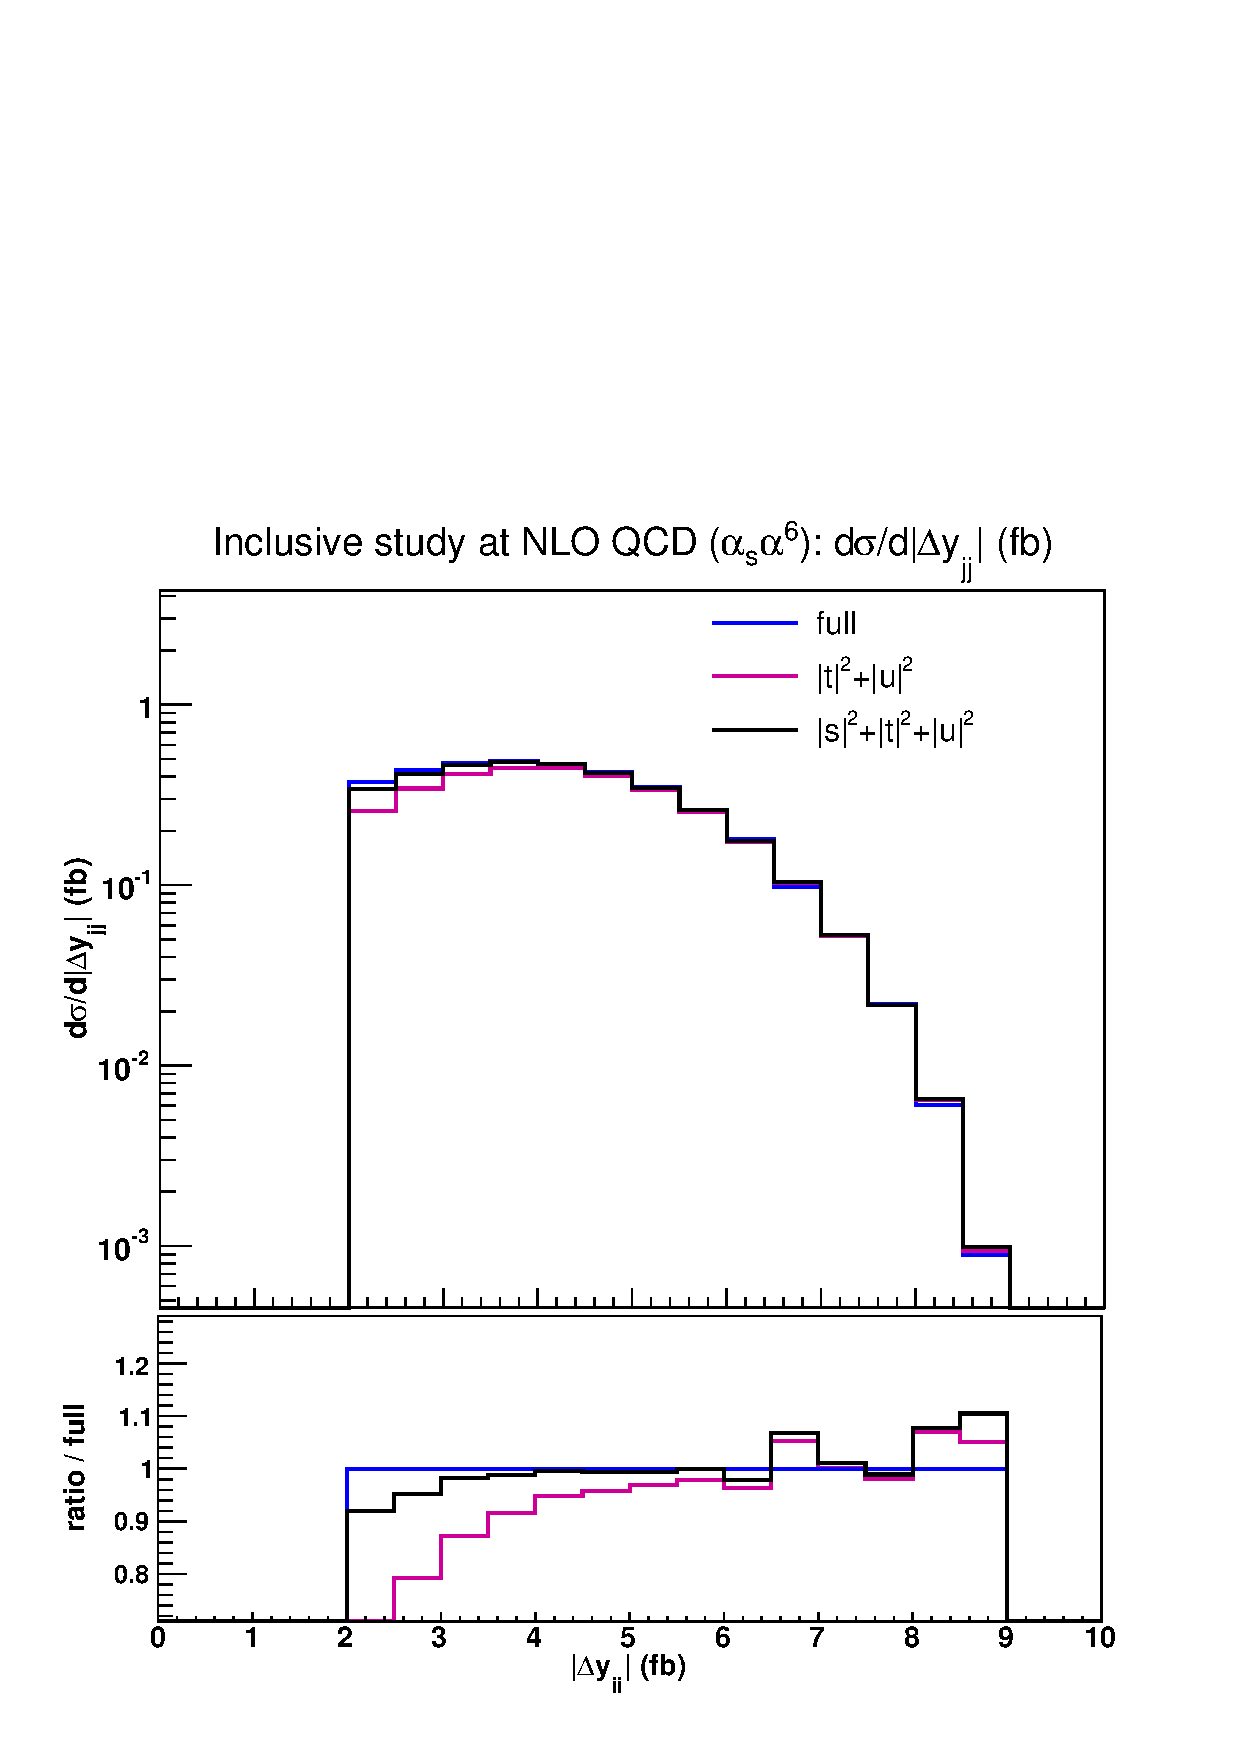
\includegraphics[scale=0.35]{figures/scanfigures/dyjj_nlo.pdf}}
\caption{NLO QCD inclusive study: distributions in $m_{jj}$ (left) and $\Delta y_{jj}$ (right), obtained with full ({\sc Recola}) and approximated ({\sc VBFNLO, Bonsay}) amplitudes at order $\mathcal{O}(\alpha_s\alpha^6)$.} \label{fig:mjjdyjj_1d_1}
\end{figure}
Focussing on the region  $200 \GeV < m_{jj} < 500 \GeV$ and $2<|\Delta y_{jj}|<2.5$, the negative discrepancy between the $|t|^2 + |u|^2$ approximation and the full computation is enhanced by up to 30 \%. The inclusion of $s$--channels cures the discrepancy in these regions; still, in the very low $m_{jj}$ a small discrepancy ($\approx$ 5 \%) becomes positive pointing out that also interferences (GP: and non--factorizable QCD corrections ?) are needed.\\
In order to investigate further the jet pair kinematics, we divide the $m_{jj},\Delta y_{jj}$ plane in 2--dimensional bins and analyze the cross--sections: in particular we compute in each bin the ratio of the approximated cross--section over the full one. In Fig.~\ref{fig:ratio2d_NLO} and Fig.~\ref{fig:mjjdyjj_2d_NLO} we show respectively the ratio $\sigma(|t|^2 + |u|^2)/\sigma(\textrm{full})$ and $\sigma(|s|^2+|t|^2 + |u|^2)/\sigma(\textrm{full})$.
\begin{figure}[h]
\centering
{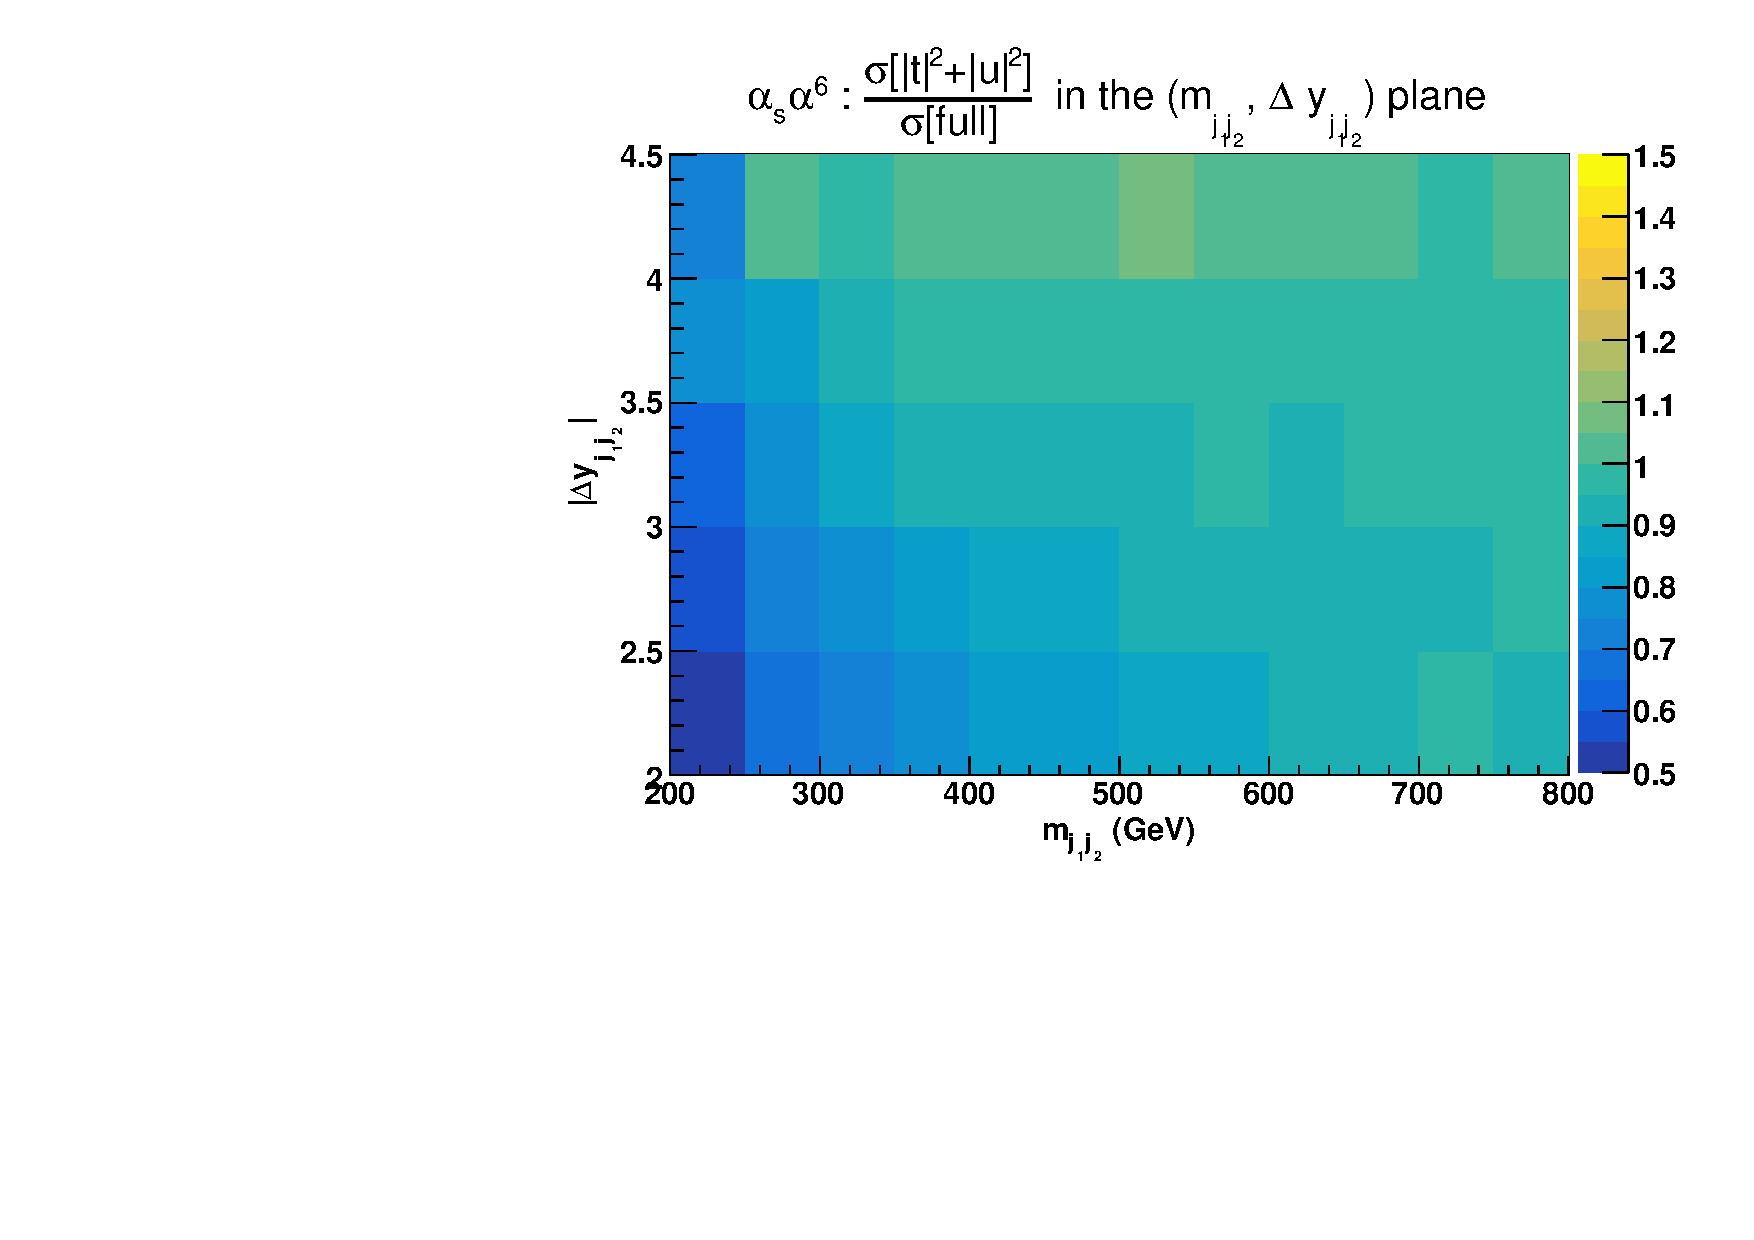
\includegraphics[scale=0.39]{figures/scanfigures/a6as_vbfnloVSrecola_tu.pdf}}
%\includegraphics[scale=0.395]{figures/scanfigures/.pdf}
\caption{Cross sections (fb) per bin of $(m_{jj},\,\Delta y_{jj})$ at NLO QCD $\mathcal{O}(\alpha_s\alpha^6)$, without any cut on the $jj$ pair kinematics: ratio of approximated squared amplitudes over the full matrix element. The approximated squared amplitudes are computed as $|\mathcal{A}|^2 \sim |t|^2 + |u|^2$. Results of {\sc Bonsay} (approximated) and {\sc Recola} (full) calculations. {\bf GP: notation to be changed, Mjj > mjj, alphas alpha} }\label{fig:ratio2d_NLO}
\end{figure}
\begin{figure}[hbt]
\centering
{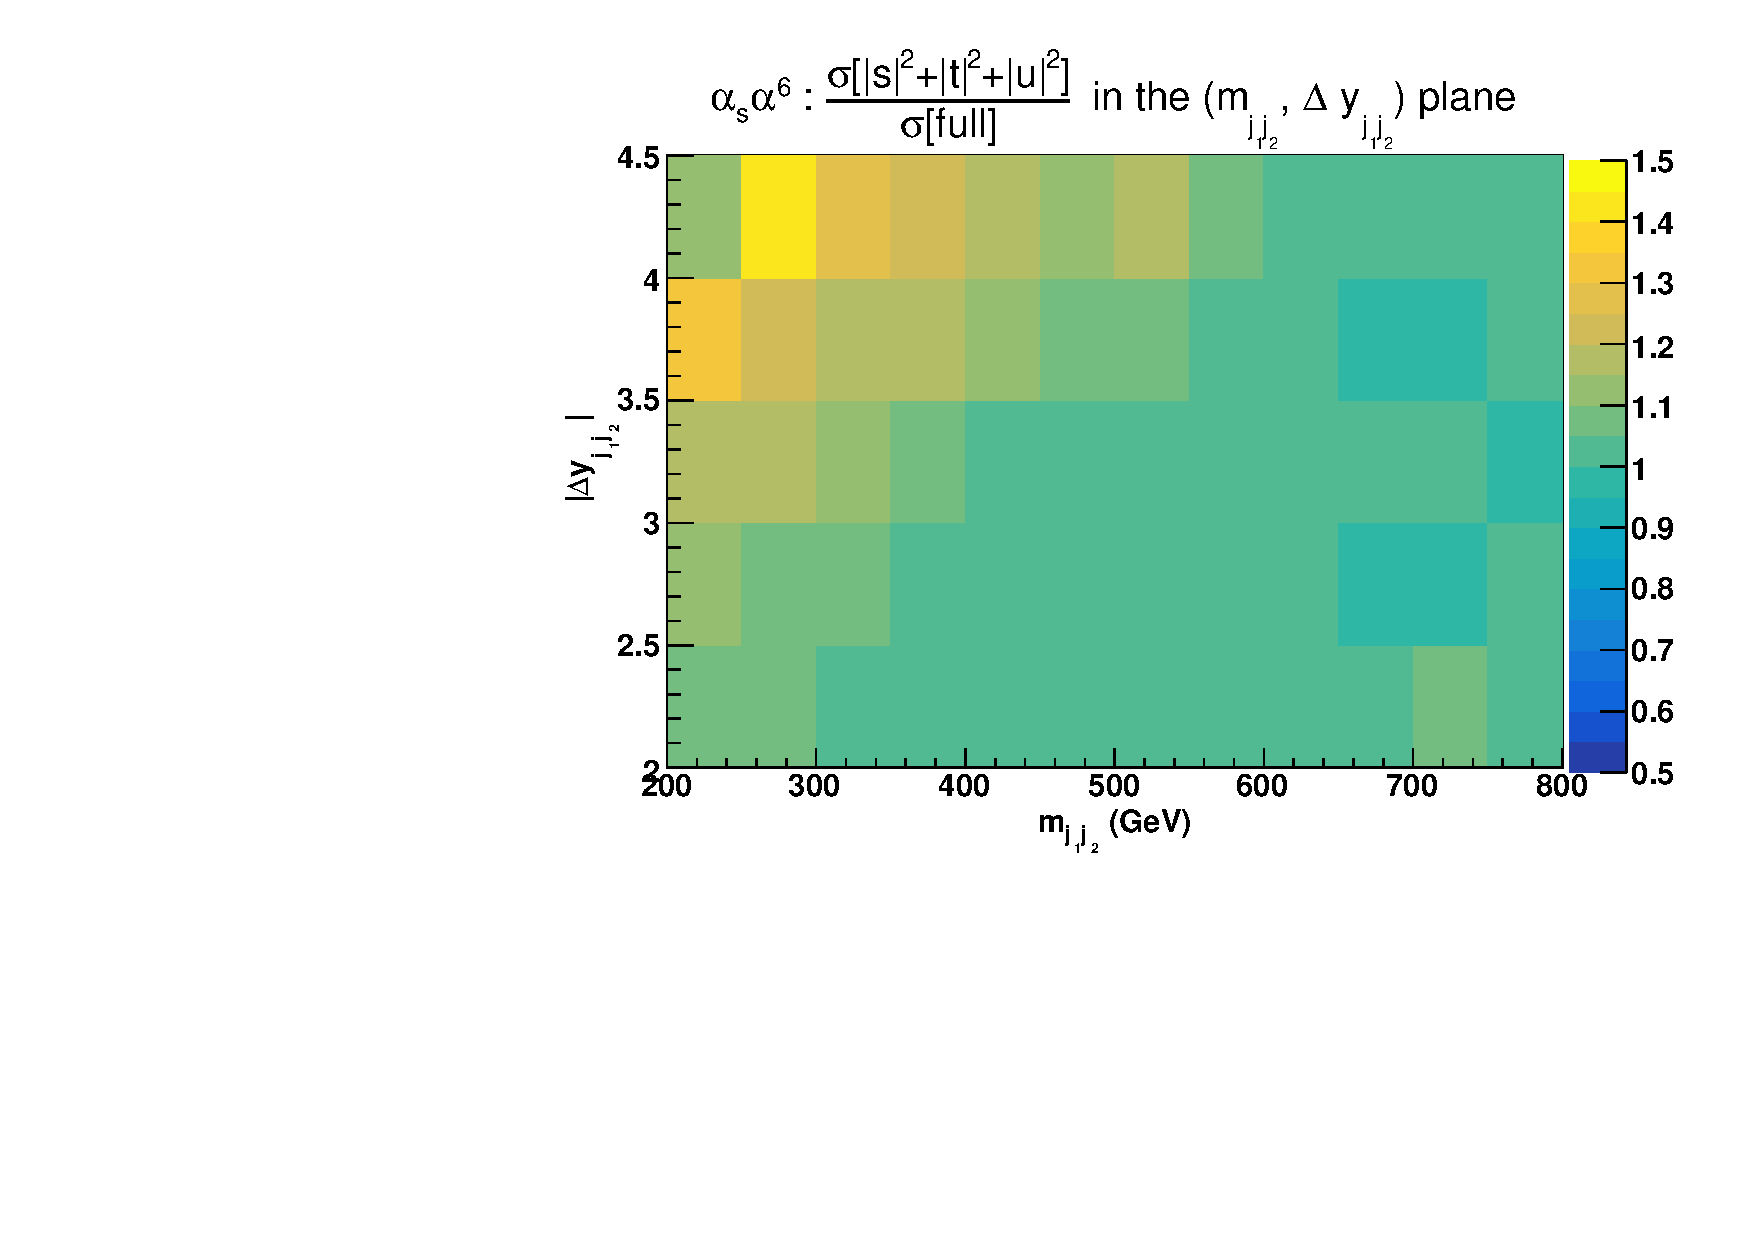
\includegraphics[scale=0.39]{figures/scanfigures/a6as_vbfnloVSrecola_stu.pdf}}
\caption{Cross section (fb) per bin of $(m_{jj},\,\Delta y_{jj})$ at NLO QCD $\mathcal{O}(\alpha_s\alpha^6)$, without any cut on the $jj$ pair kinematics:  ratio of approximated squared amplitudes over the full matrix element. The approximated squared amplitudes are computed as $|\mathcal{A}|^2 \sim |s|^2 + |t|^2 + |u|^2$. Results of {\sc VBFNLO} (approximated) and {\sc Recola} (full) calculations. {\bf GP: notation to be changed, Mjj > mjj, alphas alpha}}\label{fig:mjjdyjj_2d_NLO}
\end{figure}
As expected, in the low invariant mass--low rapidity separation region of the jet--jet pair the VBS approximation fails badly (up to 40 \% discrepancies) and the $s$--channel inclusion lead to discrepancies of at most 5 \%. However, the positive discrepancy shown in the low $m_{jj}$ region (black curve, Fig.~\ref{fig:mjjdyjj_1d_1}) can be traced back to the low $m_{jj}$, large $\Delta y_{jj}$ region of Fig.~\ref{fig:mjjdyjj_2d_NLO}, where the two leading jets have soft transverse momenta, according to the following approximation
\begin{equation}
\begin{split}
m_{jj}^2 &= 2\,p_t^{j_1}p_t^{j_2}\,(\cosh \Delta y_{jj} - \cos \Delta\phi_{jj})
&\approx 2\,p_t^{j_1}p_t^{j_2}\,\cosh \Delta y_{jj} \,\,.
\end{split}
\end{equation}
The same positive discrepancy of the $|s|^2 + |t|^2 + |u|^2$ approximation, in fact, can be seen in the low $p_t$ region of the leading jet in the left panel of Fig.~\ref{fig:mjjdyjj_1d_2}.\\
In the large invariant mass--small rapidity separation region of Fig.~\ref{fig:mjjdyjj_2d_NLO}, discrepancies at the 15 \% level are left: this can be traced back to the large $p_t$ and central rapidity region of the leading jets kinematics, shown in Fig.~\ref{fig:mjjdyjj_1d_2}. For such distributions, despite the $s$--channel inclusion, the discrepancy between the approximated and full result is about 5-10 \%.\\
In the VBS signal region the VBS approximation shows a good agreement with the full calculation.
\begin{figure}[hbt]
\centering
{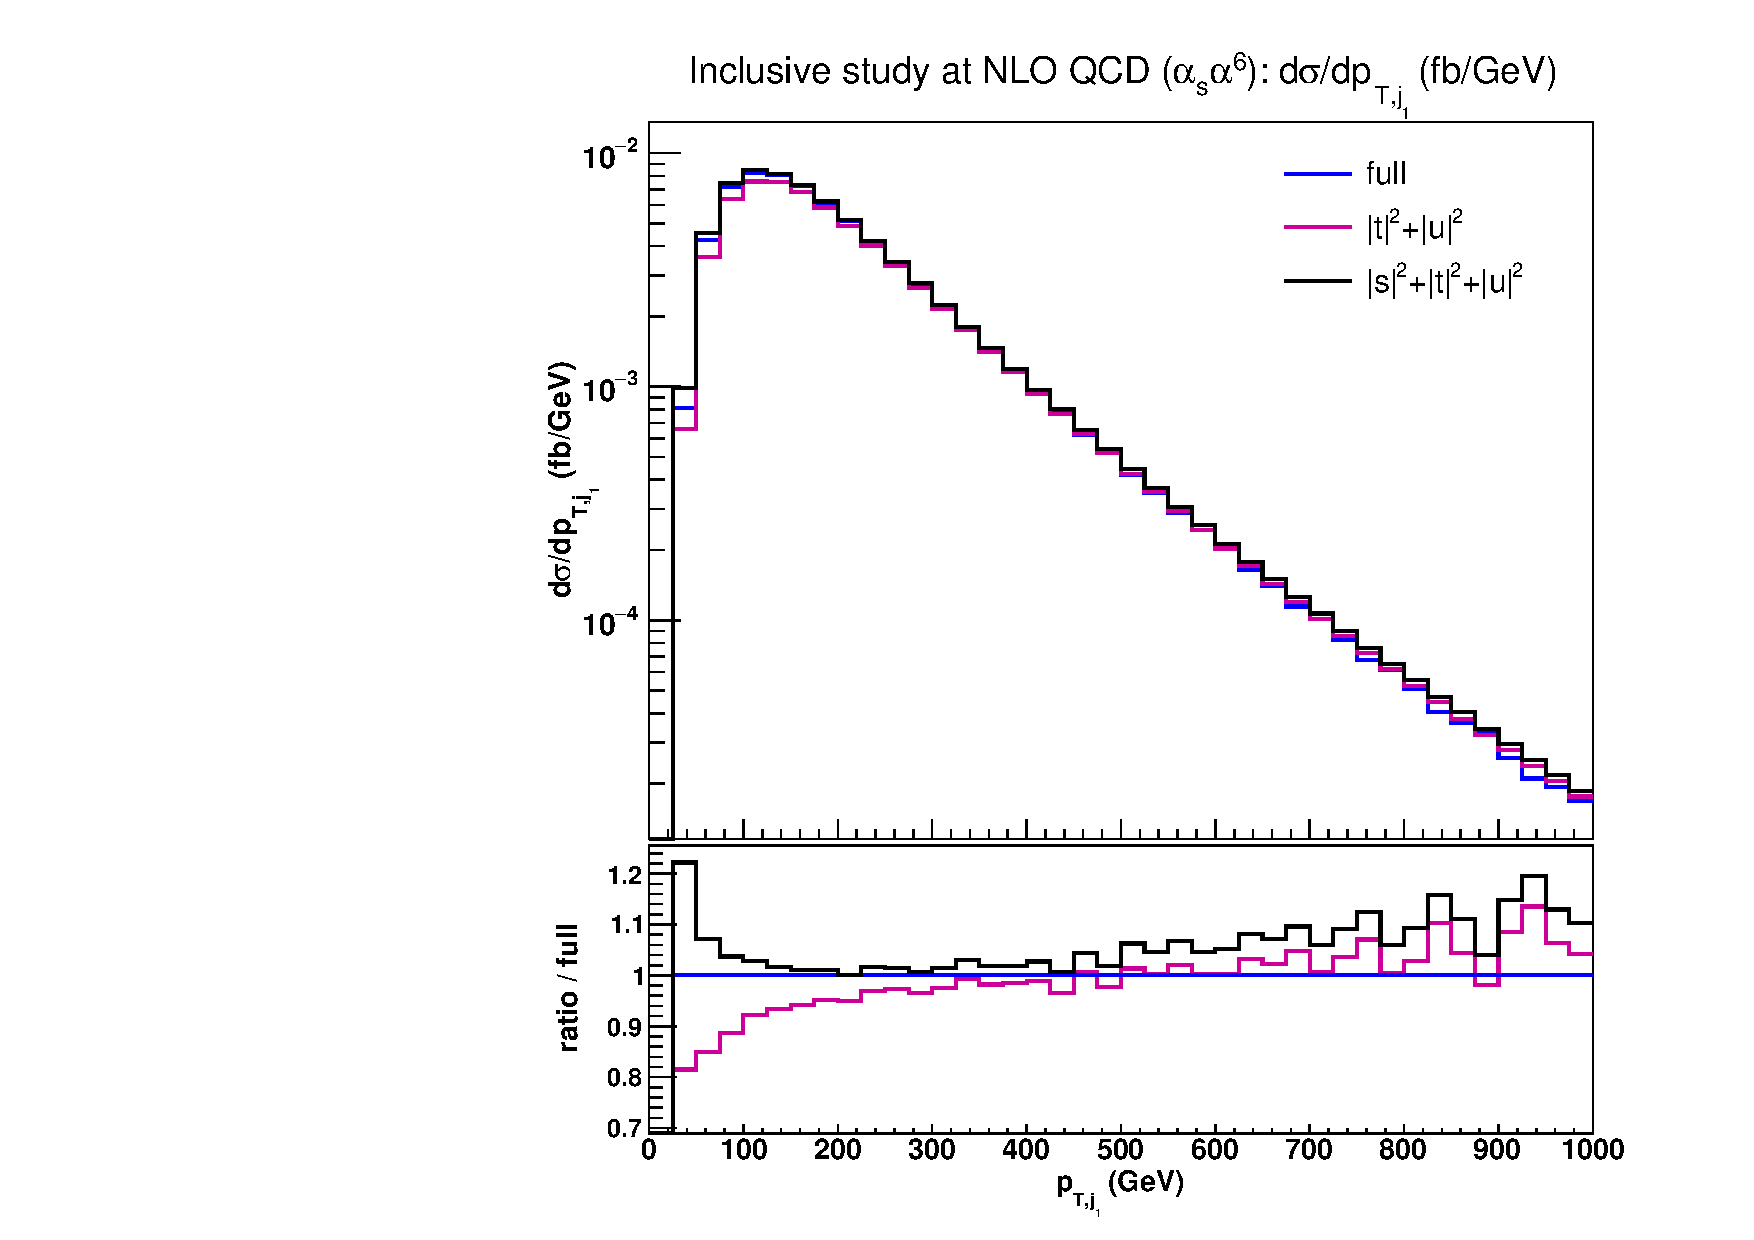
\includegraphics[scale=0.35]{figures/scanfigures/ptj1_nlo.pdf}}
{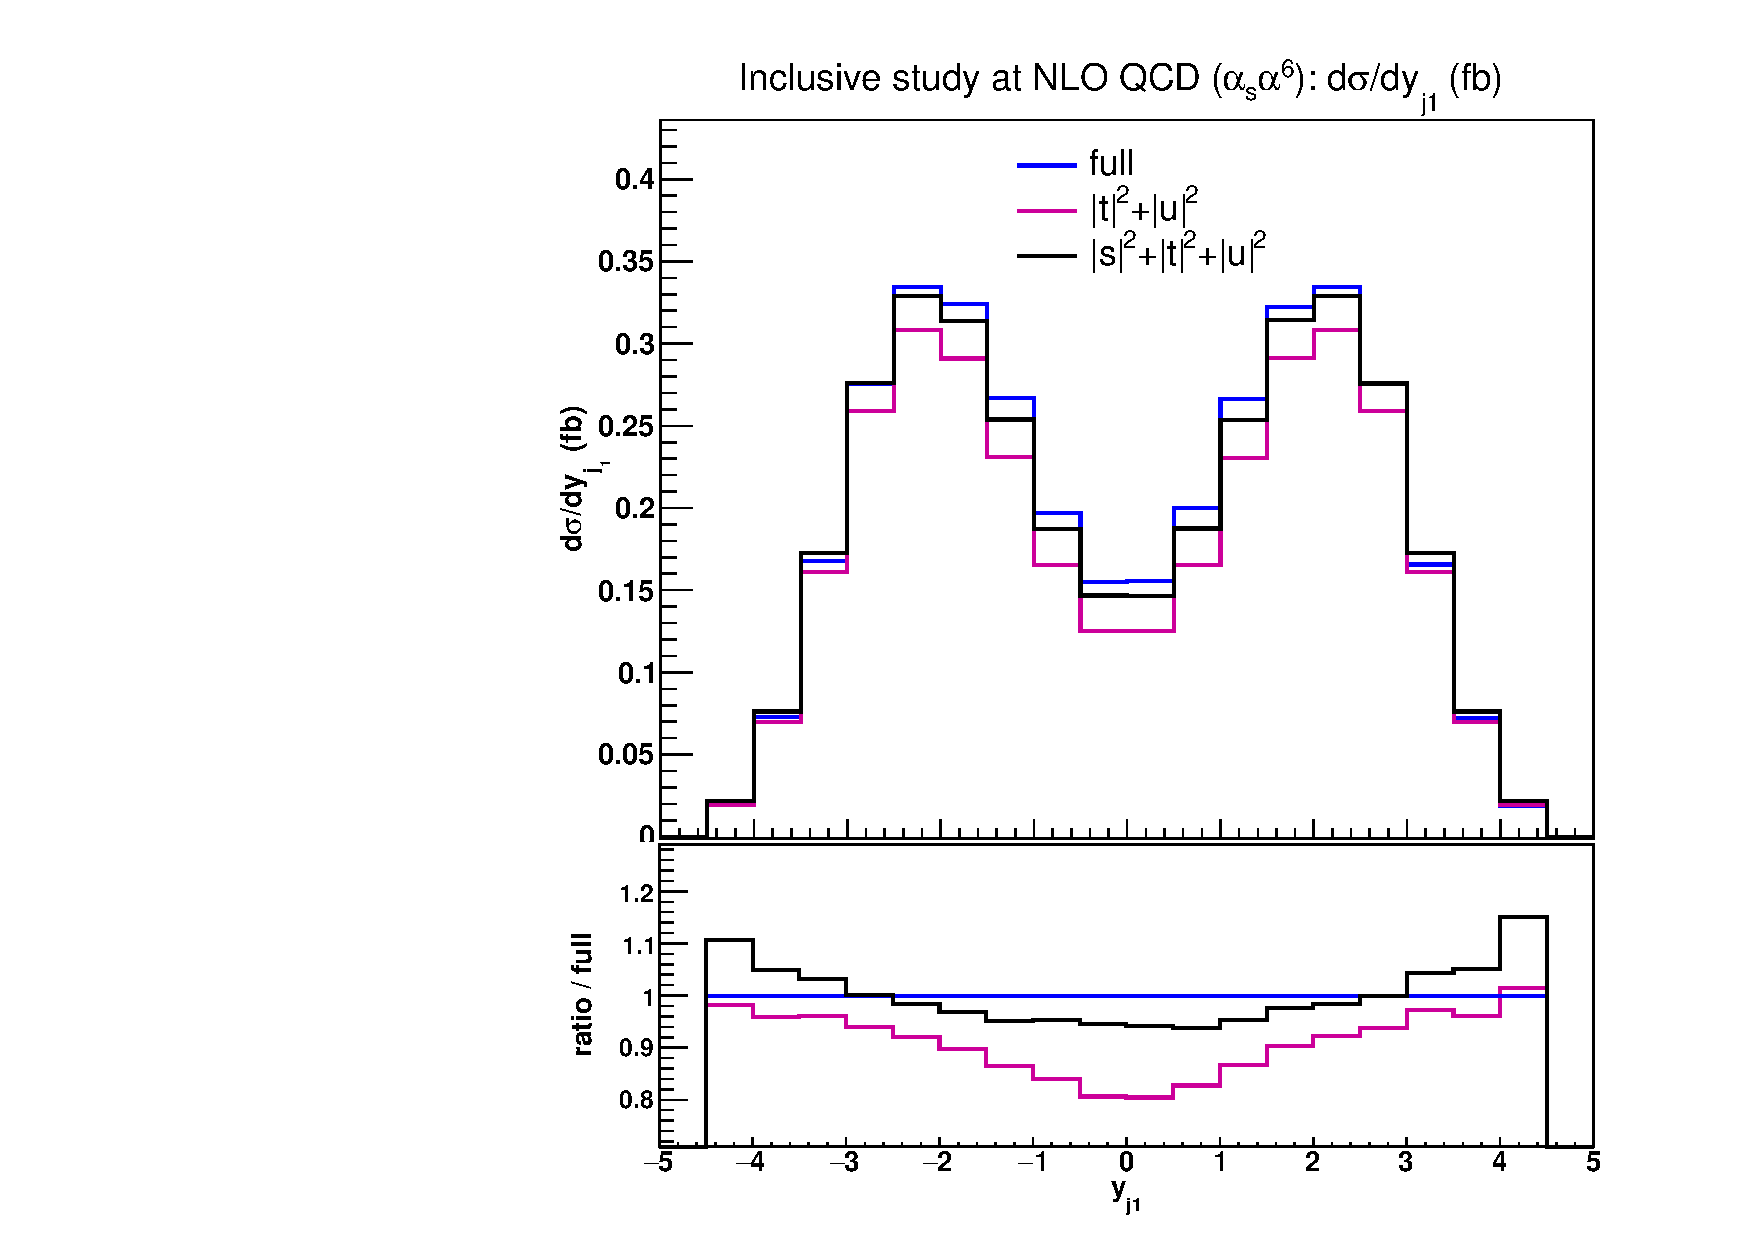
\includegraphics[scale=0.35]{figures/scanfigures/yj1_nlo.pdf}}
\caption{NLO QCD inclusive study: transverse momentum and rapidity distributions of the leading jet, obtained with full ({\sc Recola}) and approximated ({\sc VBFNLO, Bonsay}) amplitudes at order $\mathcal{O}(\alpha_s\alpha^6)$.} \label{fig:mjjdyjj_1d_2}
\end{figure}

Concerning leptonic kinematcs, we show in Fig.~\ref{fig:mjjdyjj_1d_3} the distributions of the lepton--lepton invariant mass and of the Zeppenfeld variable of the electron.
\begin{figure}[hbt]
\centering
{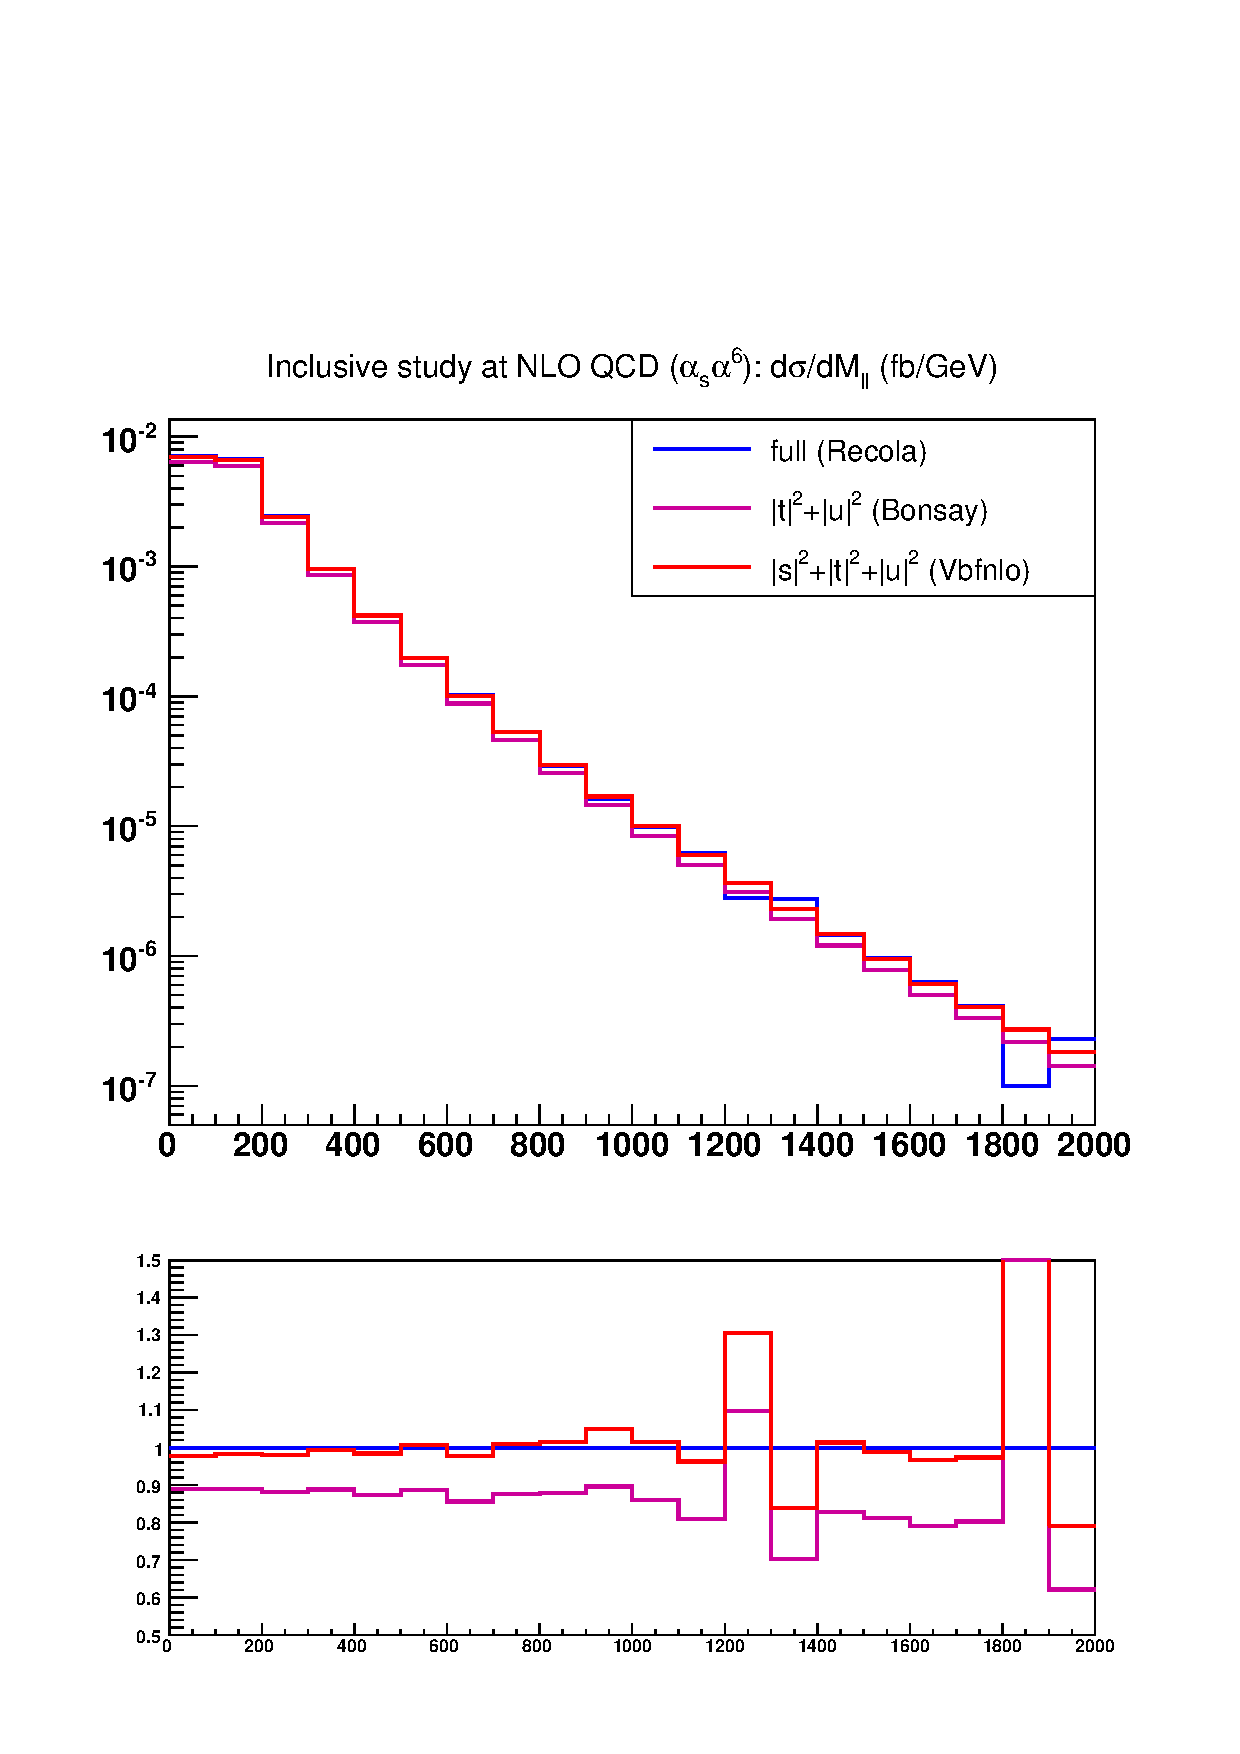
\includegraphics[scale=0.35]{figures/scanfigures/mll_nlo.pdf}}
{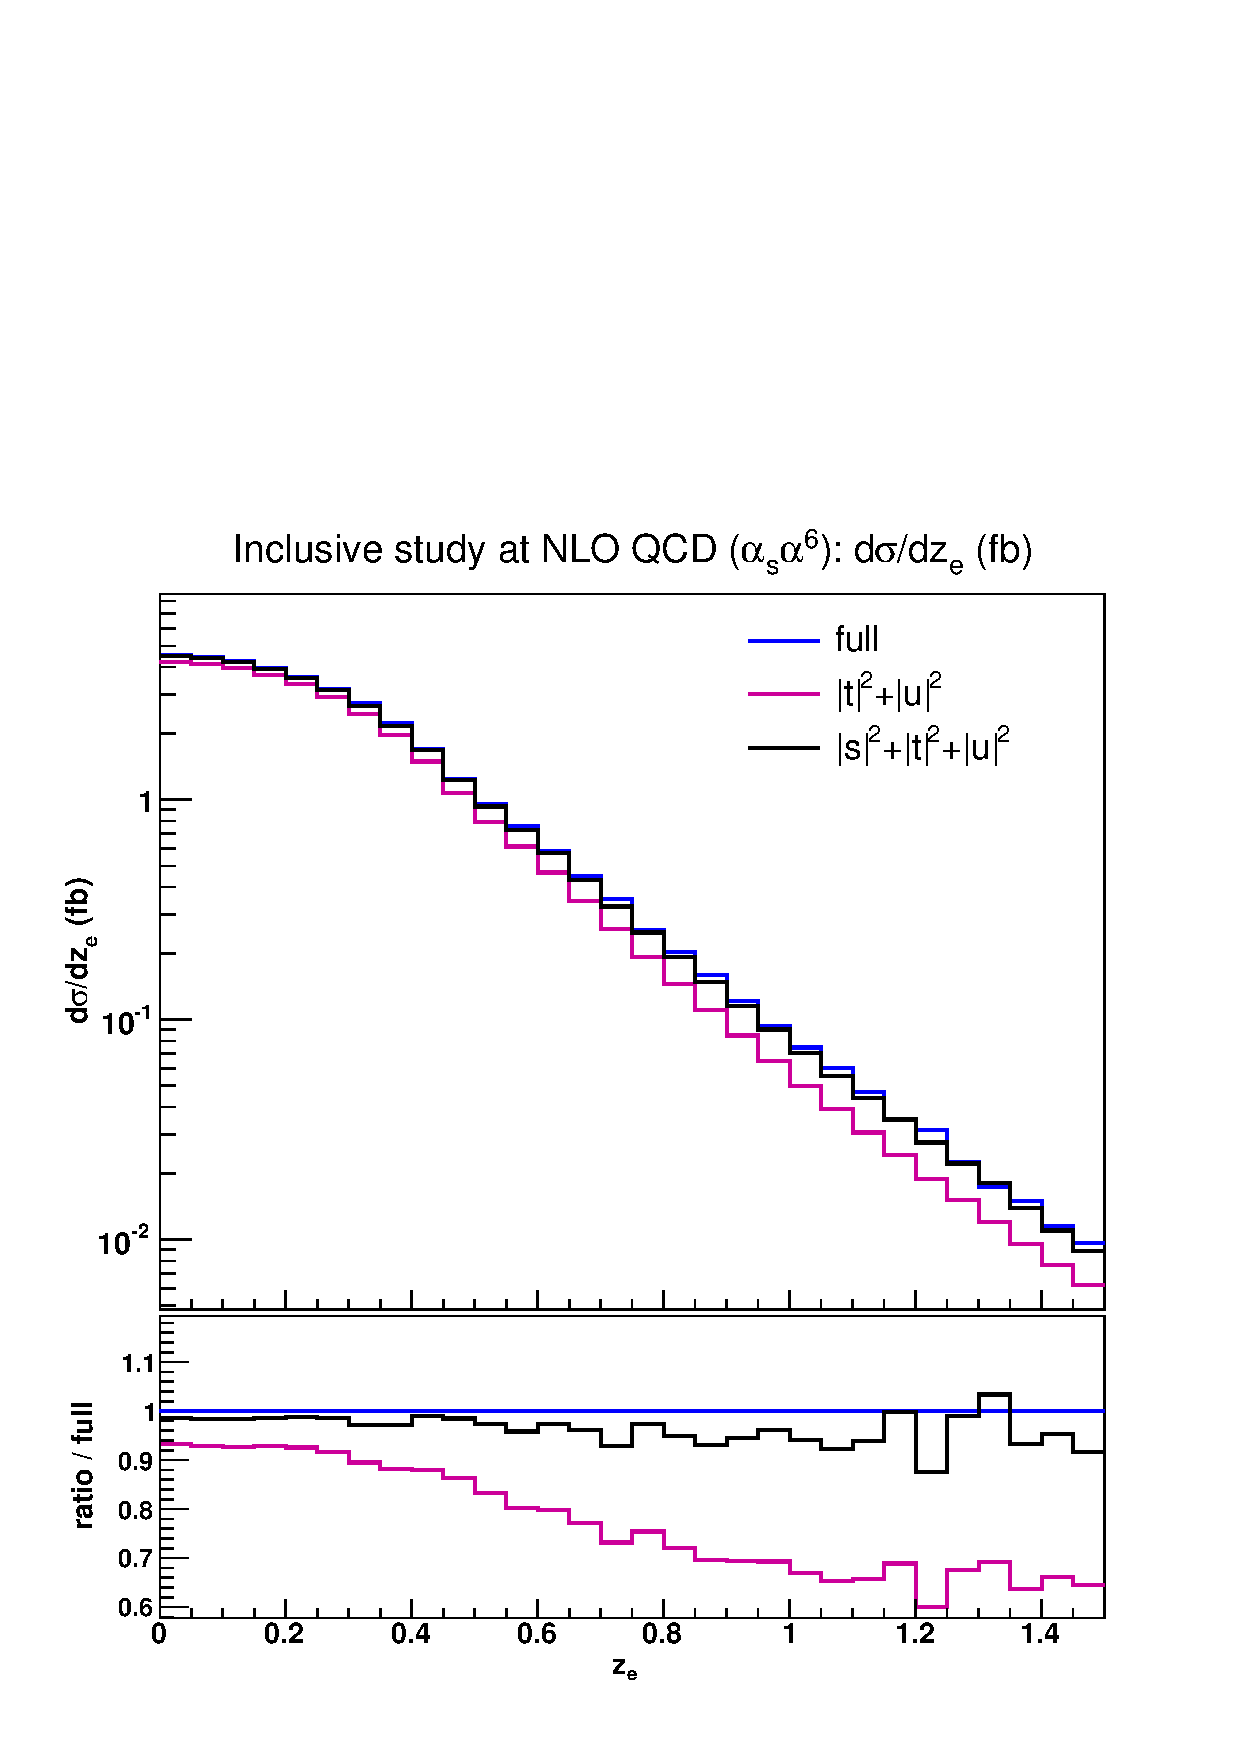
\includegraphics[scale=0.35]{figures/scanfigures/zel_nlo.pdf}}
\caption{NLO QCD inclusive study: distributions of the lepton--lepton invariant mass and the electron Zeppenfeld variable, obtained with full ({\sc Recola}) and approximated ({\sc VBFNLO, Bonsay}) amplitudes at order $\mathcal{O}(\alpha_s\alpha^6)$.} \label{fig:mjjdyjj_1d_3}
\end{figure}
{\bf GP: leptonic variables, comment further.}


In conclusion, both the loose minimum $jj$ invariant mass cut and the inclusion of QCD radiative correction make the $s$--channel contributions less suppressed than at LO, making their inclusion mandatory, in order to provide trustworthy predictions at NLO accuracy. Nevertheless, interferences and non--factorizable QCD corrections should be included to reduce the discrepancies down to the $\approx$ 1 \%  level, mainly in inclusive analyses.\\
Instead, the VBS approximation at NLO provides a good approximation of full calculations in the kinematic region where VBS contributions are dominant ($M_{jj} \gtrsim 600 \GeV$, $\Delta y_{jj} \gtrsim 3$), concerning both total cross--section and distributions.
